\documentclass[11pt,a4paper]{article}

%\usepackage[utf8]{inputenc}
\usepackage[danish]{babel}
\usepackage{enumitem}
\usepackage{array, tabularx}
\usepackage[table]{xcolor}
\usepackage{colortbl}
\usepackage{unicode-math}
\usepackage{makecell}
\usepackage{amsmath}
\usepackage{multirow}
\usepackage{hhline}
\usepackage[hidelinks]{hyperref}
\usepackage{pgfplots}
\pgfplotsset{compat=1.18}
\usepackage{graphicx}
\usepackage{subcaption}

\setlist[enumerate,1]{
    label=\mbox{},        % empty (invisible) label
    leftmargin=0pt,       % align exactly with the text
    labelsep=0pt,
    align=left,
    itemsep=1.5\baselineskip % vertical gap between Opgaver
}

\setlist[enumerate,2]{
    label=(\alph*),
    leftmargin=2em,
    labelsep=.6em,
    itemsep=\baselineskip
}

\newcommand{\opgave}[1]{\textbf{Opgave #1}}




\begin{document}
    \section{Formål}
        Formålet er at finde ud hvor hurtig reaktionerne løber af, også kaldt for reaktionshastigheden. Derfor har vi lavet en række forsøg, hvor forskellige egenskaber blev forændret.
        
    \section{Teori}
        Vi måler reaktionshastigheden ved hjælp af en forsøg med syre og svovl, \(Δt\) er den tid når man ikke kan se pletten på papiret mere. Afstanden mellem vandoverfladen skal være konstant for at man kan sammenligne resultaterne.
        \[2H^+(aq)\  +\  S_2O_3^{2-}(aq)\ →\ S(s)\ +\ SO_2(aq)\ + \ H_2O(l) \]
        
        Ændringen i koncentrationen af \(HCl\) og \([S_2O_2^{}]\) kan betragtes som 0, fordi det er så lidt. I vores tilfælde er reaktionshastigheden givet ved:
        \[v = \frac{-Δ[S_2O_3^{2-}]}{Δt} = \frac{1}{Δt} \]
        Det betyder at den sidste kolonne er også reaktionshastigheden.
        
    \section{Hypotese}
        Jeg forventer at den går hurtigere når den har en forøget koncentration. Det går også hurtigere når temperaturen er højere.
    \section{Materialer}
        Tre bægerglas, to buretter, målværktøj (stopur, termometer, etc.)\\
        Saltsyre (\(HCl\)) (0,4M), Natriumthiosulfat (\(Na_2S_2O_3\)) (0,4M)
       
        
        \begin{figure}[htbp]
          \centering
          \begin{subfigure}{0.4\linewidth}
            \includegraphics[width=\linewidth]{20250918_111422.jpg}
            \caption{Buretter og bægerglag}
            \label{fig:left}
          \end{subfigure}\hfill
          \begin{subfigure}{0.4\linewidth}
            \includegraphics[width=\linewidth]{20250918_123029.jpg}
            \caption{Reagerede løsning}
            \label{fig:right}
          \end{subfigure}
          \caption{}
          \label{fig:both}
        \end{figure}
    \section{Sikkerhedsvurdering}
        \(HCl\):\\
        \emph{ National Center for Biotechnology Information (2025). PubChem Compound Summary for CID 313, Hydrochloric Acid. Retrieved September 28, 2025 from} \url{https://pubchem.ncbi.nlm.nih.gov/compound/Hydrochloric-Acid}.\\ \\
        \(Na_2S_2O_3\):\\
        \emph{National Center for Biotechnology Information (2025). PubChem Compound Summary for CID 24477, Sodium Thiosulfate. Retrieved September 28, 2025 from} /\url{https://pubchem.ncbi.nlm.nih.gov/compound/Sodium-Thiosulfate}.
        
    \section{Sikkerhedskonklusion}
        \(Na_2S_2O_3\) en ufarlig, \(HCl\) skal ikke røres og dampen skal ikke indåndes. Derfor er en kittel og en sikkerhedsbrille stærk anbefalt.
        
    \section{Fremgangsmåde}
        Man fylder den mængde af de to substanser ind i hver en bægerglas. Derefter starter man et stopur når man blander de to kemikalier i en anden bægerglas. Så kigger man fra toppen igennem visken og stopper tiden når den er ikke synlig mere. Det gør man til all forskellige mængder.\\
        Når man opvarmer saltsyren, kan man bruge en bunsenbrænner, eller man bruger bare en vandkoger og varmer syren på den måde.
         
    \section{Data}
        
        % --- Table ---
        \begin{table}[hbp]
            \centering
            \renewcommand\arraystretch{1.2}
            \setlength{\tabcolsep}{6pt}
                \begin{tabular}{||c||c|c|c||c|c||c||c||}
                \hline \hline
                %\multicolumn{8}{|l|}{\textbf{Forsøgsrække A: Tabel til regne- og måleresultater}}\\ \hline
                \multirow{2}{*}{\makecell{Forsøg nr.}} &
                \multicolumn{3}{c|}{\makecell{Volumen (mL)}} &
                \multirow{2}{*}{\makecell{[\(\mathrm{H}^+\)]\\(mol/L)}} &
                \multirow{2}{*}{\makecell{[\(\mathrm{S_2O_3^{2-}}\)]\\(mol/L)}} &
                \multirow{2}{*}{\makecell{Reaktionstid,\\$\Delta t$ (s)}} &
                \multirow{2}{*}{\makecell{$\dfrac{1}{\Delta t}$ (s$^{-1}$)}} \\
                \cline{2-4}
                & H$_2$O & HCl & Na$_2$S$_2$O$_3$ & & & & \\ \hline \hline
                1  & 0  & 20 & 20 & 0,2 & 0,2 & 13,0 & 0,0769 \\ \hline
                2  & 5  & 20 & 15 & 0,2 & 0,15 & 17,2 & 0,0581 \\ \hline
                3  & 10 & 20 & 10 & 0,2 & 0,1 & 27,0 & 0,0370 \\ \hline
                4  & 15 & 20 & 5  & 0,2 & 0,05 & 53,4 & 0,0187 \\ \hline
                5  & 10 & 10 & 20 & 0,1 & 0,2 & 16,2 & 0,0617 \\ \hline \hline
            \end{tabular}
        \end{table}
        
        \begin{table}[ht]
            \centering
            \renewcommand\arraystretch{1.2}
            \setlength{\tabcolsep}{6pt}
            
            % Thick vertical bar before the last column:
            \begin{tabular}{||c||c|c|||c||}
                \hline\hline
                \makecell{Forsøg nr.} &
                \makecell{Temperatur, T\\(°C)} &
                \makecell{Reaktionstid, $\Delta t$\\(s)} &
                \makecell{$\dfrac{1}{\Delta t}$ (s$^{-1}$)} \\
                \hline\hline
                3 & 20 & 27,0 & 0,0370 \\ \hline
                6 & 48 & 4,8 & 0,208 \\ \hline\hline
            \end{tabular}
        \end{table}
        
        
  
    \section{Databehandling}
        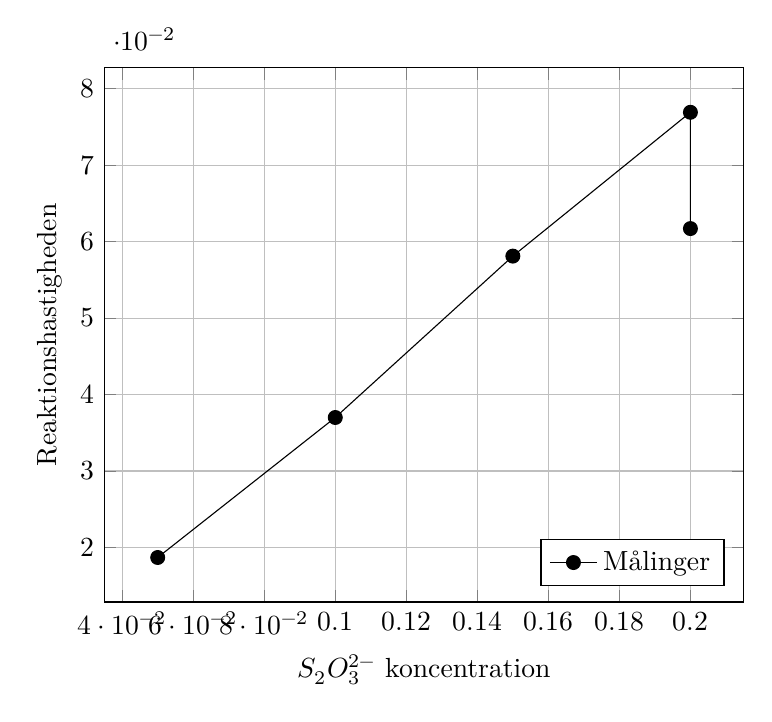
\begin{tikzpicture}
            \begin{axis}[
                width=0.8*\linewidth,
                xlabel={\(S_2O_3^{2-}\) koncentration},
                ylabel={Reaktionshastigheden},
                grid=both,
                legend pos=south east
                ]
                % Kun punkter:
                \addplot[ mark=*, mark size=2.5pt]
                coordinates {(0.2, 0.0617) (0.2, 0.0769) (0.15, 0.0581) (0.1, 0.0370) (0.05, 0.0187) };
                \addlegendentry{Målinger}
            \end{axis}
        \end{tikzpicture} \\
        Stigningen beregnes som differens af værdierne i forhold til målingerne:
        \[m = \frac{0,0617-0,0187}{0,2-0,05} = \frac{0,0430}{0,15} = 2,86\]
        Reaktionshastigheden er derfor givet ved \(v = 2,86 \frac{l}{mol·s}·[S_2O_3^{2-}]\)

        
        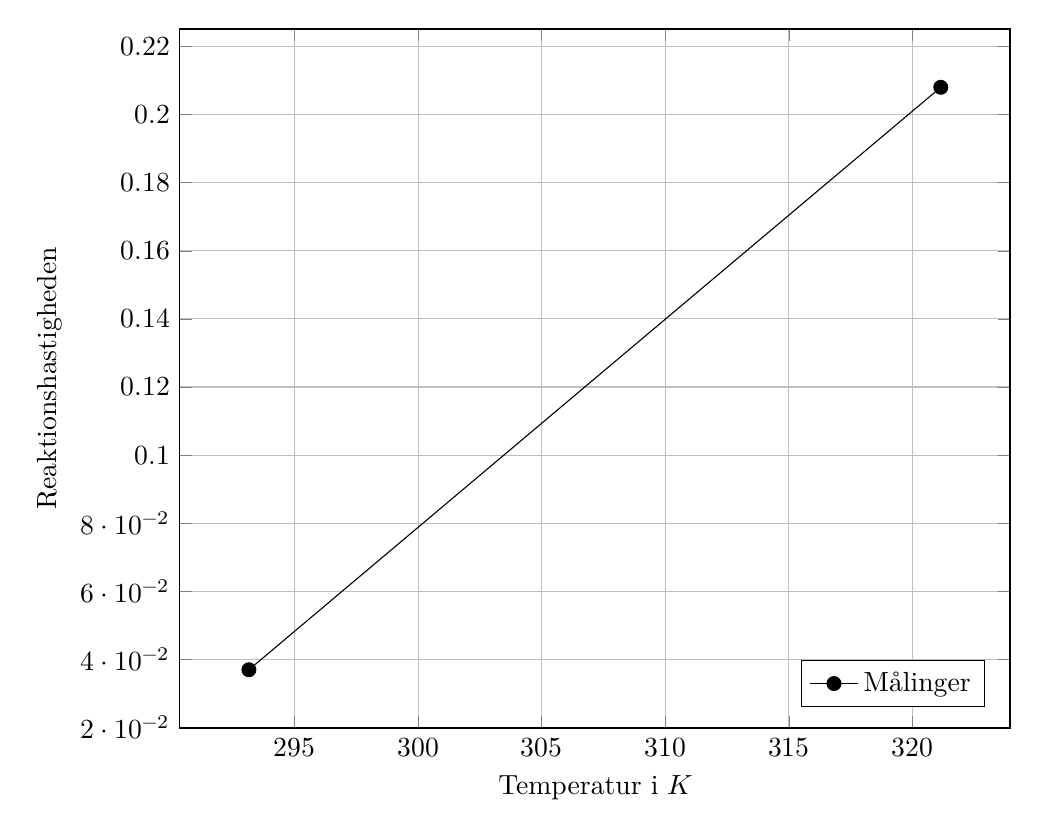
\begin{tikzpicture}
            \begin{axis}[
                width=\linewidth,
                xlabel={Temperatur i \(K\)},
                ylabel={Reaktionshastigheden},
                grid=both,
                legend pos=south east
                ]
                % Kun punkter:
                \addplot[ mark=*, mark size=2.5pt]
                coordinates {(293.15, 0.0370) (321.15, 0.208) };
                \addlegendentry{Målinger}
            \end{axis}
        \end{tikzpicture} 
        Her er det det samme, kun i afhængighed af temperaturen:
        \[v=\frac{321,15-293,15}{0,208-0,0370} = \frac{28}{0,171} = 164 \frac{K} {s} \]
    \section{Diskussion/fejlkilder}
        Jeg ved ikke hvordan jeg skal indtage forsøg 5 i stigningen, fordi det har en anden koncentration af \(HCl\). \\
        En fejlkilde er den upræcise måling med stopur, men i grafen ser det ud til at være en lille fejl. \\
        Jeg er ikke sikker hvordan man kan forstå den resultat med temperaturen.
        
        
    \section{Konklusion}
        Reaktionshastigheden er som forventet afhængig af de to størrelser, Temperatur og koncentration. Hypotesen var altså rigtig!
\end{document}
